\documentclass{beamer}
%\usepackage[margin=1in]{geometry}
\usepackage{amsthm,amsmath,amsfonts,hyperref,graphicx,color,multicol}
\usepackage{enumitem,tikz}

%%%%%%%%%%
%Beamer Template Customization
%%%%%%%%%%
\setbeamertemplate{navigation symbols}{}
\setbeamertemplate{theorems}[ams style]
\setbeamertemplate{blocks}[rounded]

\definecolor{Blu}{RGB}{43,62,133} % UWEC Blue
\setbeamercolor{structure}{fg=Blu} % Titles

%Unnumbered footnotes:
\newcommand{\blfootnote}[1]{%
	\begingroup
	\renewcommand\thefootnote{}\footnote{#1}%
	\addtocounter{footnote}{-1}%
	\endgroup
}


%%%%%%%%%%
%Custom Commands
%%%%%%%%%%
\newcommand{\R}{\mathbb{R}}
\newcommand{\veca}{\mathbf{a}}
\newcommand{\vecb}{\mathbf{b}}
\newcommand{\vece}{\mathbf{e}}
\newcommand{\vecu}{\mathbf{u}}
\newcommand{\vecv}{\mathbf{v}}
\newcommand{\vecw}{\mathbf{w}}
\newcommand{\vecx}{\mathbf{x}}
\newcommand{\zerovector}{\mathbf{0}}

\newcommand{\ds}{\displaystyle}

\newcommand{\fn}{\insertframenumber}

\newcommand{\rank}{\operatorname{rank}}
\newcommand{\adj}{\operatorname{adj}}

\newcommand{\blank}[1]{\underline{\hspace*{#1}}}


%%%%%%%%%%
%Custom Theorem Environments
%%%%%%%%%%
\theoremstyle{definition}
\newtheorem{exercise}{Exercise}
\newtheorem{question}[exercise]{Question}
\newtheorem*{defn}{Definition}
\newtheorem*{exa}{Example}
\newtheorem*{disc}{Group Discussion}
\newtheorem*{nb}{Note}
\newtheorem*{recall}{Recall}
\renewcommand{\emph}[1]{{\color{blue}\texttt{#1}}}

\definecolor{Gold}{RGB}{237, 172, 26}
%Statement block
\newenvironment{statementblock}[1]{%
	\setbeamercolor{block body}{bg=Gold!20}
	\setbeamercolor{block title}{bg=Gold}
	\begin{block}{\textbf{#1.}}}{\end{block}}





\begin{document}
	\title{Math 324: Linear Algebra}
	\subtitle{Section 4.1: Vectors in $\R^n$}
	\author{Mckenzie West}
	\date{Last Updated: \today}
\begin{frame}
\maketitle
\end{frame}

\begin{frame}{\insertframenumber}
%	\begin{block}{\textbf{Last Time.}}
%	\begin{itemize}[label=--]
%		\item More Properties of Determinants
%		\item The Adjoin of a Matrix
%		\item Cramer's Rule
%	\end{itemize}
%	\end{block}
	\begin{block}{\textbf{Today.}}
		\begin{itemize}[label=--]
			\item Vectors in 2-d
			\item Vectors in $n$-dimensional space
		\end{itemize}
	\end{block}
\end{frame}
\begin{frame}{\fn}
	\begin{exercise}
		Geometrically (tail-to-tip) and algebraically compute each of the following for $\vec{u}=(-2,1.5)$ and $\vec{v}=(1,6)$.
			\begin{enumerate}[label=(\alph*)]
				\item $\vec{u}-\vec{v}$
				\item $3\vec{v}$
				\item $\frac{1}{2}\vec{u}+\vec{v}$
			\end{enumerate}
	\end{exercise}
\end{frame}
\begin{frame}{\fn}
	\begin{statementblock}{Theorem 4.1}
		Let $\vec{u}$, $\vec{v}$, and $\vec{w}$ be vectors in the plane and let $c$ and $d$ be scalars.  Then the following are true	
			\begin{enumerate}[label=\textbf{\arabic*.}]
				\item $\vec{u}+\vec v$ is a vector in the the plane\hfill \emph{(additive closure)}
				\item $\vec u+\vec v=\vec v+\vec u$\hfill \emph{(commutativity of addition)}
				\item $(\vec u +\vec v)+\vec w = \vec u+(\vec v + \vec w)$\hfill\emph{(associativity of addition)}
				\item $\vec u +(0,0)= \vec u$\hfill\emph{(additive identity)}
				\item $\vec u+(-\vec u)=(0,0)$\hfill\emph{(additive inverse)}
				\item $c\vec u$ is a vector in the plane \hfill\emph{(scalar closure)}
				\item $c(\vec u+\vec v)=c\vec u+c\vec v$\hfill\emph{(distributivity)}
				\item $(c+d)\vec u = c\vec u + d\vec u$\hfill\emph{(distributivity)}
				\item $c(d\vec u)=(cd)\vec u$\hfill \hfill\emph{(associativity of scalars)}
				\item $1(\vec u)=\vec u$\hfill \emph{(multiplicative identity)}
			\end{enumerate}
	\end{statementblock}
\end{frame}
\begin{frame}{\fn}
	\begin{exercise}
		Use the algebraic definitions of vector addition and scalar multiplication to prove properties \textbf{2.} and \textbf{9.} of Theorem 4.1:
	\begin{enumerate}[label=--]
		\item[\textbf{2.}] $\vec u+\vec v=\vec v+\vec u$
		\item[\textbf{9.}] $c(d\vec u)=(cd)\vec u$
	\end{enumerate}
	\end{exercise}
\end{frame}

\begin{frame}{\fn}
	\begin{defn}
		An \emph{$n$-dimensional vector} is an ordered list of $n$ numbers--an \emph{$n$-tuple}--$\vec x=(x_1,x_2,\dots,x_n)$, that represents a terminal point of an arrow from the origin in \emph{$n$-dimensional space}.  Denote $n$-dimensional space by $\R^n$ (the book uses $R^n$).
	\end{defn}
	\begin{nb}
		It sure is hard to imagine what $4$-dimensional vectors look like but fortunately we have a very concrete algebraic representation.
	\end{nb}
	\begin{defn}
		Two vectors in $\R^n$ are equal if and only if their corresponding components are equal.
	\end{defn}
\end{frame}
\begin{frame}{\fn}
	\begin{defn}
		The \emph{standard operations in $\R^n$} are the following definitions of vector addition and scalar multiplication:
		
		Let $\vec u= (u_1,u_2,\dots,u_n)$ and $\vec v=(v_1,v_2,\dots,v_n)$ be vectors in $\R^n$ and let $c$ be a scalar. We define the \emph{sum} of $\vec u$ and $\vec v$ as:
			\[\vec u+\vec v=(u_1+v_1,u_2+v_2,\dots,u_n+v_n).\]
		Define the \emph{scalar multiple} of $\vec u$ by $c$ as:
			\[c\vec u=(cu_1,cu_2,\dots,cu_n).\]
\end{defn}
\end{frame}
\begin{frame}{\fn}
	\begin{defn} 		
		The \emph{negative} of $\vec u$ is defined as:
		\[-\vec u = -1(\vec u)=(-u_1,-u_2,\dots,-u_n),\]
		and the \emph{difference} of $\vecu$ and $\vecv$ is:
		\[\vecu-\vecv=\vec u+(-\vecv)=(u_1-v_1,u_2-v_2,\dots,u_n-v_n).\]
		
		Lastly, the \emph{zero vector} in $\R^n$ is the point at the origin, \[\vec 0=(0,0,\dots,0).\]
	\end{defn}
\end{frame}
\begin{frame}{\fn}
	\begin{exercise}
		Let $\vec u = (-2, 4, 0, -4)$, $\vec v= (0, 5, 5, 4)$, $\vec w = (1, -4, 3, 3)$ and $c=-2$, compute:
	\begin{enumerate}[label=(\alph*)]
		\item $\vec u+\vec v$
		\item $c\vec w$
		\item $2\vec w-\vec v$
	\end{enumerate}
	\end{exercise}
\end{frame}
\begin{frame}{\fn}
	\begin{statementblock}{Theorem 4.2}
		Let $\vec{u}$, $\vec{v}$, and $\vec{w}$ be vectors in $\R^n$ and let $c$ and $d$ be scalars.  Then the following are true	
		\begin{enumerate}[label=\textbf{\arabic*.}]
			\item $\vec{u}+\vec v$ is a vector in the the plane\hfill \emph{(additive closure)}
			\item $\vec u+\vec v=\vec v+\vec u$\hfill \emph{(commutativity of addition)}
			\item $(\vec u +\vec v)+\vec w = \vec u+(\vec v + \vec w)$\hfill\emph{(associativity of addition)}
			\item $\vec u +\vec 0= \vec u$\hfill\emph{(additive identity)}
			\item $\vec u+(-\vec u)=\vec 0$\hfill\emph{(additive inverse)}
			\item $c\vec u$ is a vector in the plane \hfill\emph{(scalar closure)}
			\item $c(\vec u+\vec v)=c\vec u+c\vec v$\hfill\emph{(distributivity)}
			\item $(c+d)\vec u = c\vec u + d\vec u$\hfill\emph{(distributivity)}
			\item $c(d\vec u)=(cd)\vec u$\hfill \hfill\emph{(associativity of scalars)}
			\item $1(\vec u)=\vec u$\hfill \emph{(multiplicative identity)}
		\end{enumerate}
	\end{statementblock}
\end{frame}
\begin{frame}{\fn}
	\begin{exercise}
		Let $\vec u=(-1,3,1)$, $\vec v=(5,-5,6)$, and $\vec w=(3,7,4)$.
		Find $\vec x$ given the equation:
		\begin{enumerate}[label=(\alph*)]
			\item $\vec x = 3\vec u+4\vec v-7\vec w$
			\item $\frac{1}{2}(\vec w+\vec x)=2\vec u-\vec v$
		\end{enumerate}
	\end{exercise}
\end{frame}
\begin{frame}{\fn}
	\begin{defn}
		We call the zero vector, $\vec 0$, in $\R^n$ the \emph{additive identity} and the negative, $-\vec u$, the \emph{additive inverse} of $\vec u$. 
		
		These vectors have very special properties as outlined in the following Theorem.
	\end{defn}
	\begin{statementblock}{Theorem 4.3}
		Let $\vec u\in\R^n$ and $c$ a scalar.  Then the following are true:
		\begin{enumerate}[label=\textbf{\arabic*.}]
			\item The additive identity is unique.  (If $\vec u+\vec v=\vec u$, then $\vec v=\vec 0$.)
			\item The additive inverse is unique.  (If $\vec u+\vec v=\vec 0$, then $\vec v=-\vec u$.)
			\item $0\vec u=\vec 0$
			\item $c\vec 0=\vec 0$
			\item If $c\vec u=\vec 0$ then $c=0$ or $\vec v=\vec 0$.
			\item $-(-\vecu)=\vec u$
		\end{enumerate}
	\end{statementblock}
\end{frame}
\begin{frame}{\fn}
	\begin{exercise}
		Prove property \textbf{1.} of Theorem 4.3:
		\begin{enumerate}[label=--]
			\item[\textbf{1.}] If $\vec u+\vec v=\vec u$, then $\vec v=\vec 0$.
		\end{enumerate}
		Challenge: Prove this without using the fact that $\vec u,\vec v\in\R^n$.  Instead just use properties from Theorem 4.2.
	\end{exercise}
\end{frame}

\begin{frame}{\fn}
\begin{block}{\textbf{Brain Break.}}
	Do you have any pets? If so what kind, how many, what are their names? If not, do you want any?
	\begin{center}
		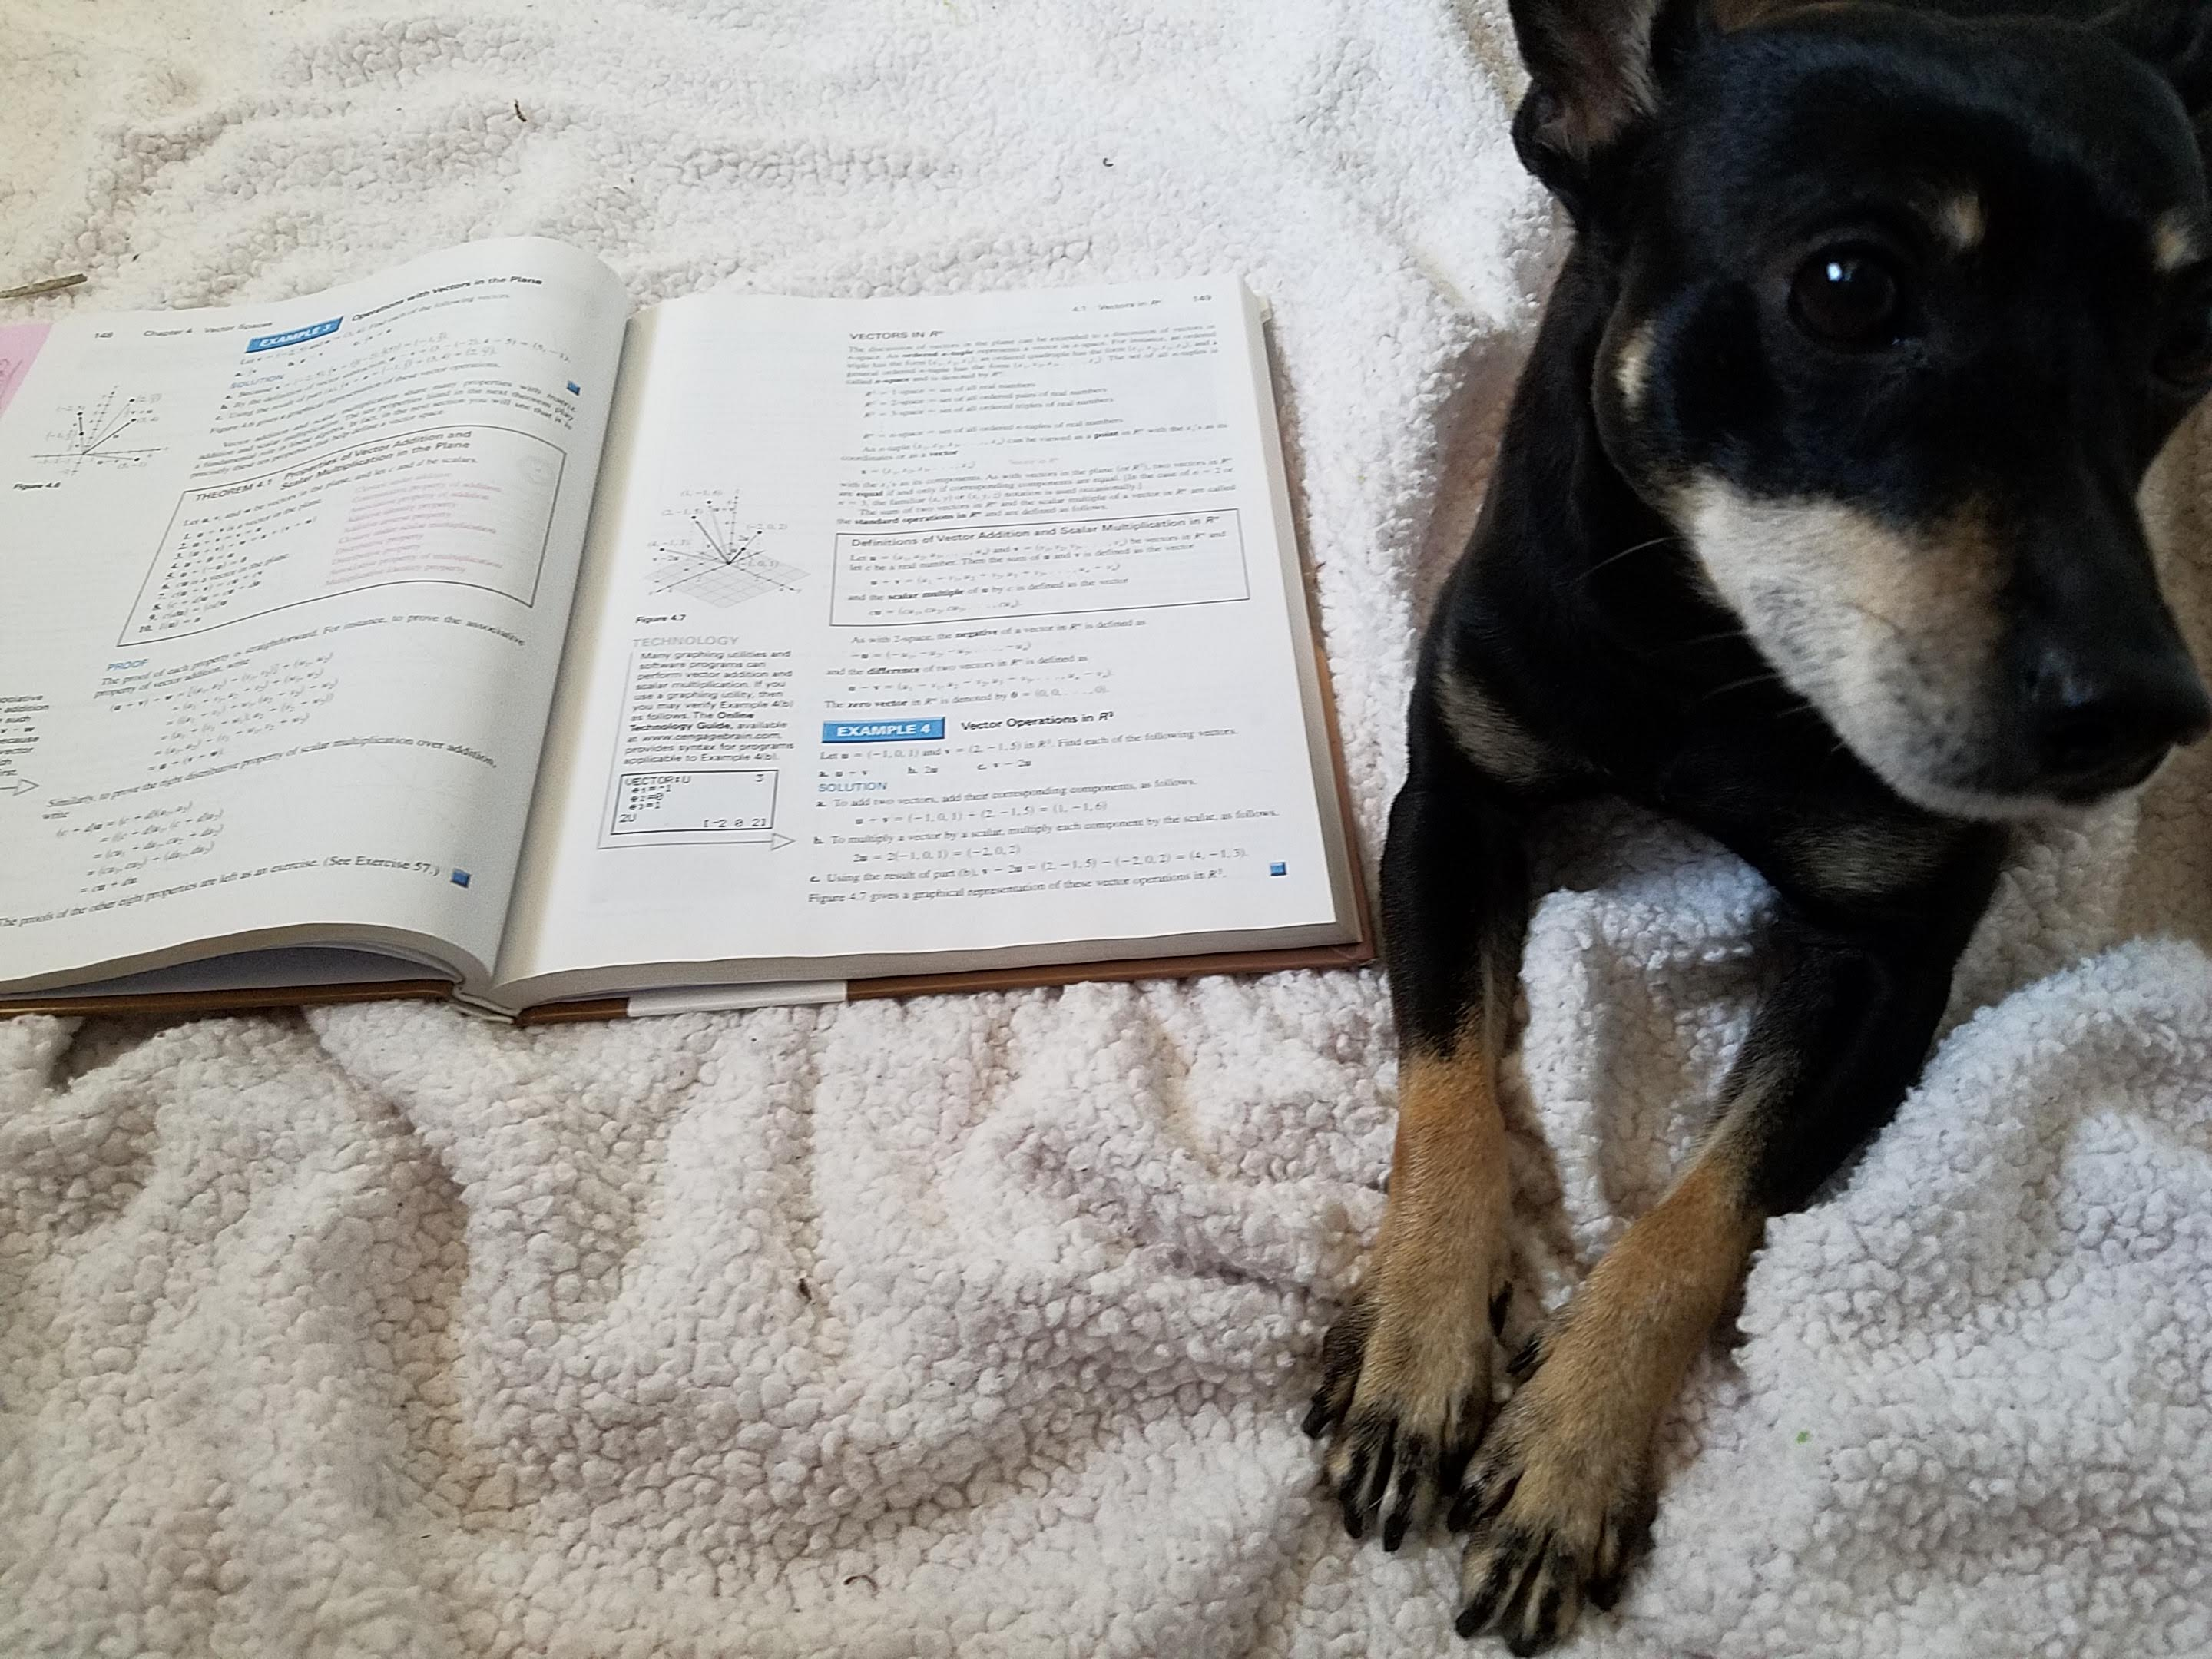
\includegraphics[width=2in]{images/s4-1_Pepper}
		
		This is my dog, Pepper, studying up on Section 4.1.
	\end{center}
\end{block}
\end{frame}

\begin{frame}{\fn}
	\begin{exercise}
		Complete the proof of property \textbf{3.} of Theorem 4.3 by justifying each step using Theorem 4.2 or properties of real numbers.
		\begin{proof}
			Let $\vec u\in\R^n$. Notice that,
			\begin{eqnarray}
			0\vec u&=&(0+0)\vec u\\
			0\vec u &=&0\vec u+0\vec u.
			\end{eqnarray}
			Then we get, $ 
			0\vec u+(-0\vec u)=(0\vec u+ 0\vec u)+(-0\vec u).$ \hfill(3)\\ \stepcounter{equation}
			Therefore,
			\begin{eqnarray}
			\vec 0&=&0\vec u+(0\vec u+(-0\vec u))\\
			\vec 0&=&0\vec u+\vec 0\\
			\vec 0&=&0\vec u.
			\end{eqnarray}
		\end{proof}
	\end{exercise}
\end{frame}
\begin{frame}{\fn}
	\begin{defn}
		A \emph{linear combination} of the vectors $\vec u_1,\vec u_2,\dots,\vec u_n\in\R^n$ is a vector of the form
			\[\vec x = c_1\vec u_1+c_2\vec u_2+\dots+c_n\vec u_n,\]
		where $c_1,c_2,\dots,c_n$ are scalars.
	\end{defn}
	\begin{exa}
		The vector $\vec x=(-13,23,-3)$ is a linear combination of $\vec u_1=(-3,1,1)$, $\vec u_2=(0,-4,-2)$ and $\vec u_3=(-3,12,-6)$ because
		
			\[\vec x=3\vec u_1-\vec u_2+\frac{4}{3}\vec u_3.\]
	\end{exa}
\end{frame}
\begin{frame}{\fn}
	\begin{exercise}
		Write $\vec x=(3,2)$ as a linear combination of $\vec u=(-1,1)$ and $\vec v=(3,4)$, if possible.
	\end{exercise}
	\begin{exercise}
		Prove that the zero vector, $\vec 0$, can be written as a linear combinination of the vectors $\vec u_1,\vec u_2,\dots,\vec u_m\in\R^n$. 
		
		Hint: Don't over-think this one, but do make sure to reference Theorems 4.2 and 4.3 as needed.
	\end{exercise}\pause
	\begin{defn}
		We call $\vec 0=0\vec u_1+0\vec u_2+\cdots+0\vec u_m$ the \emph{trivial solution}.  Any other solution is called a \emph{nontrivial solution}.
	\end{defn}
\end{frame}
\begin{frame}{\fn}
	\begin{exercise}\label{exercise:linearindependence}
		Is there a nontrivial way of writing $\vec 0$ as a linear combination of:
		\begin{enumerate}[label=(\alph*)]
			\item $\vec u=(-1,  7,  0)$, $\vec v=(-1,  5,  0)$, and $\vec w=(-4,  6,  0)$?
			\item $\vec u_1=(7,  6,  2)$, $\vec u_2=(2,  2,  0)$, and $\vec u_3=(0,  7,  -2)$?
			\item $\vec u_1=(7,  6,  2)$, $\vec u_2=(2,  2,  0)$, $\vec u_3=(0,  7,  -2)$, and $\vec u_4=(3,2,1)$?
		\end{enumerate}
	\end{exercise}
	\begin{exercise}
		Prove that every vector $\vec x=(x_1,x_2,x_3)\in\R^3$ can be written as a linear combination of $\vec u_1$, $\vec u_2$ and $\vec u_3$ as in Exercise \ref{exercise:linearindependence} part (b).
		
		Is the same true for the vectors in part (a)? Why or why not?
	\end{exercise}
\end{frame}









%\begin{frame}{\fn}
%		\begin{defn}
%			A \emph{vector in the plane} is a directed line segment with initial point at the origin and terminal point at $(x_1,x_2)$.
%			\begin{center}
%				\includegraphics[width=1.5in]{images/vector}
%			\end{center}
%			Note that the only distinguishing feature of a vector is its terminal point, so we can denote vectors via the \emph{ordered pair},
%				\[\vec{x}=(x_1,x_2).\]
%			Make sure to draw an arrow over the name of a vector to distinguish it from individual \emph{components}---$x_1$ and $x_2$.
%		\end{defn}
%\end{frame}
%\begin{frame}{\fn}
%	\begin{exercise}
%		Sketch the line segment in the plane that represents:
%			\begin{enumerate}[label=(\alph*)]
%				\item $(-4,3)$
%				\item $(1,0)$
%				\item $(0,-1)$
%			\end{enumerate}
%	\end{exercise}
%\end{frame}
%\begin{frame}{\fn}
%	\begin{defn}
%		Two vectors $\vec{u}=(u_1,u_2)$ and $\vec{v}=(v_1,v_2)$ are \emph{equal} if $u_1=v_1$ and $u_2=v_2$.
%		
%		\emph{Vector Addition} is determined geometrically using a tip-to-tail technique:
%		
%			\begin{minipage}{1in}
%			\includegraphics[width=1in]{images/vector_add1}
%			\end{minipage}\hfill$\rightarrow$\hfill
%			\begin{minipage}{1in}
%			\includegraphics[width=1in]{images/vector_add2}
%			\end{minipage}\hfill$\rightarrow$\hfill
%			\begin{minipage}{1.1in}
%				\includegraphics[width=1.1in]{images/vector_add3}
%			\end{minipage}
%	\end{defn}
%	\begin{exercise}
%		Use this definition of vector addition to compute $(1,3)+(4,-1)$.  Do you get the same thing if you compute $(4,-1)+(1,3)$? 
%		
%		Why or why not?
%	\end{exercise}
%\end{frame}
%\begin{frame}{\fn}
%	\begin{defn}
%		Algebraically \emph{vector addition} is defined component-wise.  If $\vec{u}=(u_1,u_2)$ and $\vec{v}=(v_1,v_2)$, then
%			\[\vec{u}+\vec{v}=(u_1+v_1,u_2+v_2).\]
%	\end{defn}
%\end{frame}

\end{document}

